\subsubsection*{Zadanie~8.9.}
\begin{mathfigure*}
    \coordinate (A) at (-2, -0.4);
    \coordinate (B) at (1, -0.4);
    \coordinate (C) at (2, 0.4);
    \coordinate (D) at (-1, 0.4);
    \coordinate (E) at (-2, 2.6);
    \coordinate (F) at (1, 2.6);
    \coordinate (G) at (2, 3.4);
    \coordinate (H) at (-1, 3.4);
    \coordinate (I) at ($(A)!0.5!(G)$);
    \coordinate (S) at ($(A)!0.5!(C)$);
    \draw[dotted] (G) -- (S);
    \draw[dotted] (A)  -- (C);
    \draw[dashed] (D) -- (H);
    \drawrightangle{B--S--C};
    \drawrightangle[angle radius=0.3cm]{G--S--D};
    \draw[ForestGreen, thick] (D) -- (B) -- (C) -- (G);
    \draw[ForestGreen, thick] (G) -- (B);
    \draw[dashed, ForestGreen, thick] (G) -- (D);
    \draw[dashed, ForestGreen, thick] (C) -- (D);
    \draw (A) -- node[below]{\(x\)} (B) -- node[below, sloped]{\(x\)} (C);
    \draw[dashed] (C) -- (D) -- (A);
    \draw (E) -- (F) -- (G) -- (H) -- cycle;
    \draw (A) -- (E);
    \draw (B) -- (F);
    \draw (C) -- node[right]{\(x\)} (G);
    \fillpoint*{A}[\(A\)][below left];
    \fillpoint*{B}[\(B\)][below right];
    \fillpoint*{C}[\(C\)][above right];
    \fillpoint*{D}[\(D\)][above left];
    \fillpoint*{E}[\(E\)][above left];
    \fillpoint*{F}[\(F\)][above];
    \fillpoint*{G}[\(G\)][above right];
    \fillpoint*{H}[\(H\)][above left];
    \fillpoint*{I}[\(I\)][above left];
    \fillpoint*{S}[\(S\)][below];
\end{mathfigure*}
Rozważmy sześcian \(ABCDEFGH\) i~czworościan \(BCDG\). Kąty dwuścienne między następującymi parami ścian:
\begin{itemize}
    \item \(BCD\) i~\(BCG\)
    \item \(BCD\) i~\(CDG\)
    \item \(BCG\) i~\(CDG\)
\end{itemize}
są proste, ponieważ te ściany zawierają się w~ścianach sześcianu, które są do siebie prostopadłe. Natomiast kąty dwuścienne pomiędzy parami ścian
\begin{itemize}
    \item \(BCG\) i~\(BDG\)
    \item \(BCD\) i~\(BDG\)
    \item \(CDG\) i~\(BDG\)
\end{itemize}
są ostre, ponieważ kąt \(\angle{CSG}\) jest ostry i~analogicznie dla pozostałych ścian. Środek sfery opisanej na tym czworościanie jest środkiem sfery opisanej na sześcianie, czyli środkiem sześcianu i~widzimy, że leży poza czworościanem.
\subsubsection*{Zadanie~8.10.}
Wybieramy spośród wszystkich trójkątów o~wierzchołkach leżących na pewnej sferze o~środku \(Q\) dowolny rozwartokątny trójkąt \(XYZ\). Niech \(P\) leży wewnątrz tego trójkąta. Niech \(W\) będzie punktem przecięcia prostej \(PQ\) ze sferą. Wtedy czworościan \(XYZW\) spełnia warunki zadania, ponieważ ściana \(XYZ\) jest trójkątem rozwartokątnym, a~odcinek \(PW\) wraz z~punktem \(Q\) leży wewnątrz czworościanu.
\subsubsection*{Zadanie~8.11.}
\begin{mathfigure*}
    \coordinate (A) at (-2, -0.4);
    \coordinate (B) at (1, -0.4);
    \coordinate (C) at (2, 0.4);
    \coordinate (D) at (-1, 0.4);
    \coordinate (E) at (-2, 3.4);
    \coordinate (F) at (1, 3.4);
    \coordinate (G) at (2, 4.2);
    \coordinate (H) at (-1, 4.2);
    \coordinate (P) at ($(B)!0.5!(C)$);
    \coordinate (Q) at ($(C)!0.5!(D)$);
    \coordinate (R) at ($(G)!0.5!(D)$);
    \coordinate (S) at ($(G)!0.5!(B)$);
    \draw[dotted] (F) -- (H);
    \draw[dashed] (D) -- (H);
    \draw[ForestGreen, thick] (D) -- (B) -- (C) -- (G);
    \draw[ForestGreen, thick] (G) -- (B);
    \draw[dashed, ForestGreen, thick] (G) -- (D);
    \draw[dashed, ForestGreen, thick] (C) -- (D);
    \draw (A) -- (B) -- (C);
    \draw[dashed] (C) -- (D) -- (A);
    \draw (E) -- (F) -- (G) -- (H) -- cycle;
    \draw (A) -- (E);
    \draw (B) -- (F);
    \draw (C) -- (G);
    \draw[dashed, Magenta, thick] (P) -- (Q) -- (R) -- (S) -- cycle;
    \fillpoint*{A}[\(A\)][below left];
    \fillpoint*{B}[\(B\)][below right];
    \fillpoint*{C}[\(C\)][above right];
    \fillpoint*{D}[\(D\)][above left];
    \fillpoint*{E}[\(E\)][above left];
    \fillpoint*{F}[\(F\)][above];
    \fillpoint*{G}[\(G\)][above right];
    \fillpoint*{H}[\(H\)][above left];
    \fillpoint*{P}[\(P\)][below right];
    \fillpoint*{Q}[\(Q\)][above left];
    \fillpoint*{R}[\(R\)][above left];
    \fillpoint*{S}[\(S\)][below right];
\end{mathfigure*}
Rozważamy prostopadłościan \(ABCDEFGH\) o~podstawie kwadratu \(ABCD\), że \(BDHF\) jest kwadratem, czyli \(BD = DH = HF = FB\), oraz czworościan \(BCDG\). Niech płaszczyzna przechodzi przez środki odcinków \(BC\), \(CD\), \(GD\), \(GB\), oznaczone odpowiednio jako \(P\), \(Q\), \(R\), \(S\). Wtedy
\begin{gather*}
    PQ = \frac{1}{2} \cdot BD\\
    QR = \frac{1}{2} \cdot CG = \frac{1}{2} \cdot DH\\
    RS = \frac{1}{2} \cdot BD\\
    SP = \frac{1}{2} \cdot CG = \frac{1}{2} \cdot BF
\end{gather*}
Zatem \(PQ = QR = RS = SP\), czyli \(PQRS\) jest kwadratem, a~czworościan \(BCDG\) nie był foremny (gdyż, na przykład, \(BD \neq BC\)).
\subsubsection*{Zadanie~8.12.}
\begin{mathfigure*}
    \coordinate (A) at (-2, -0.4);
    \coordinate (B) at (1, -0.4);
    \coordinate (C) at (2, 0.4);
    \coordinate (D) at (-1, 0.4);
    \coordinate (E) at (-2, 2.6);
    \coordinate (F) at (1, 2.6);
    \coordinate (G) at (2, 3.4);
    \coordinate (H) at (-1, 3.4);
    \draw[dashed] (D) -- (H);
    \draw[ForestGreen, thick] (D) -- (B) -- (C) -- (E);
    \draw[ForestGreen, thick] (E) -- (B);
    \draw[dashed, ForestGreen, thick] (E) -- (D);
    \draw[dashed, ForestGreen, thick] (C) -- (D);
    \draw (A) -- (B) -- (C);
    \draw[dashed] (C) -- (D) -- (A);
    \draw (E) -- (F) -- (G) -- (H) -- cycle;
    \draw (A) -- (E);
    \draw (B) -- (F);
    \draw (C) -- (G);
    \fillpoint*{A}[\(A\)][below left];
    \fillpoint*{B}[\(B\)][below right];
    \fillpoint*{C}[\(C\)][above right];
    \fillpoint*{D}[\(D\)][below];
    \fillpoint*{E}[\(E\)][above left];
    \fillpoint*{F}[\(F\)][above];
    \fillpoint*{G}[\(G\)][above right];
    \fillpoint*{H}[\(H\)][above left];
\end{mathfigure*}
\subsubsection*{Zadanie~8.13.}
Niech w~podstawie będzie trójkąt o~jednym kącie rozwartym mniejszym od \(120\degree\). Wtedy wewnątrz tego trójkąta leży punkt Torricellego-Fermata, z~którego każdy bok widać po kątem \(120\degree\):
\begin{figure}[H]
    \centering
    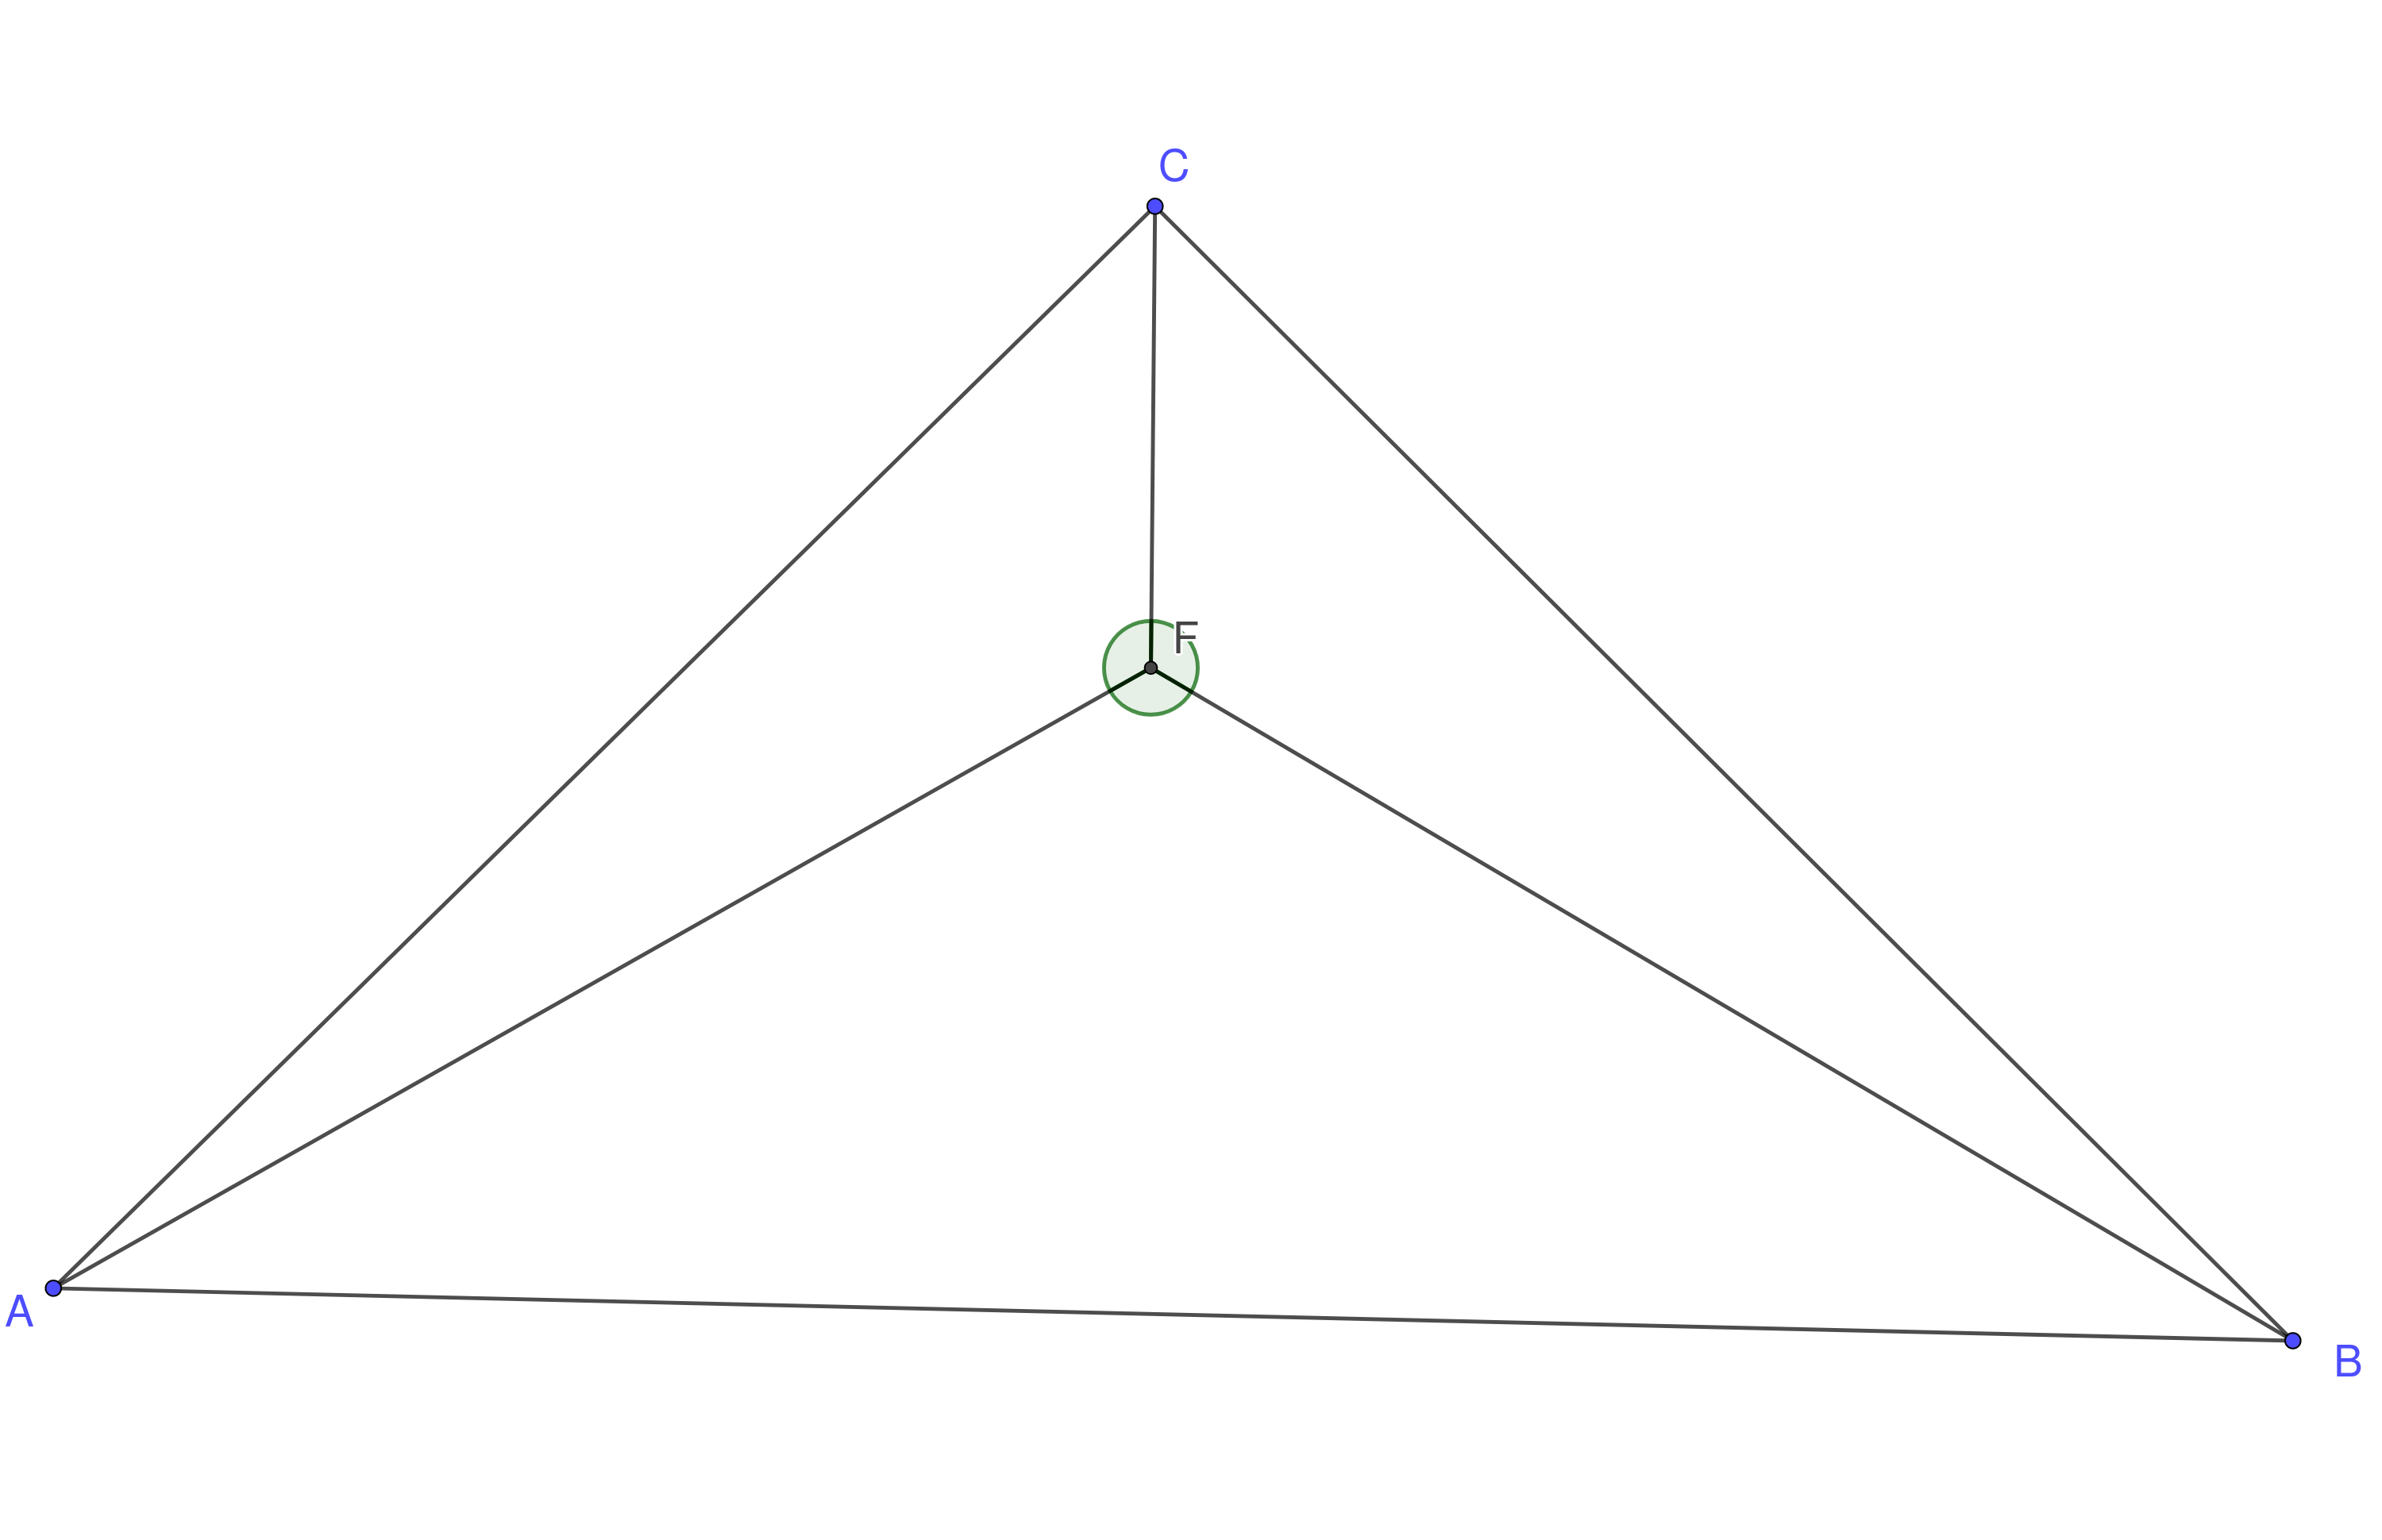
\includegraphics[scale=0.7]{img/2021_02_11/13/plane.png}
\end{figure}
\noindent
Jeśli teraz ten punkt \(F\) podniesiemy ponad płaszczyznę o~odpowiedni, bardzo niewielki dystans \(\varepsilon\), to wszystkie kąty ścian bocznych dalej będą rozwarte:
\begin{figure}[H]
    \centering
    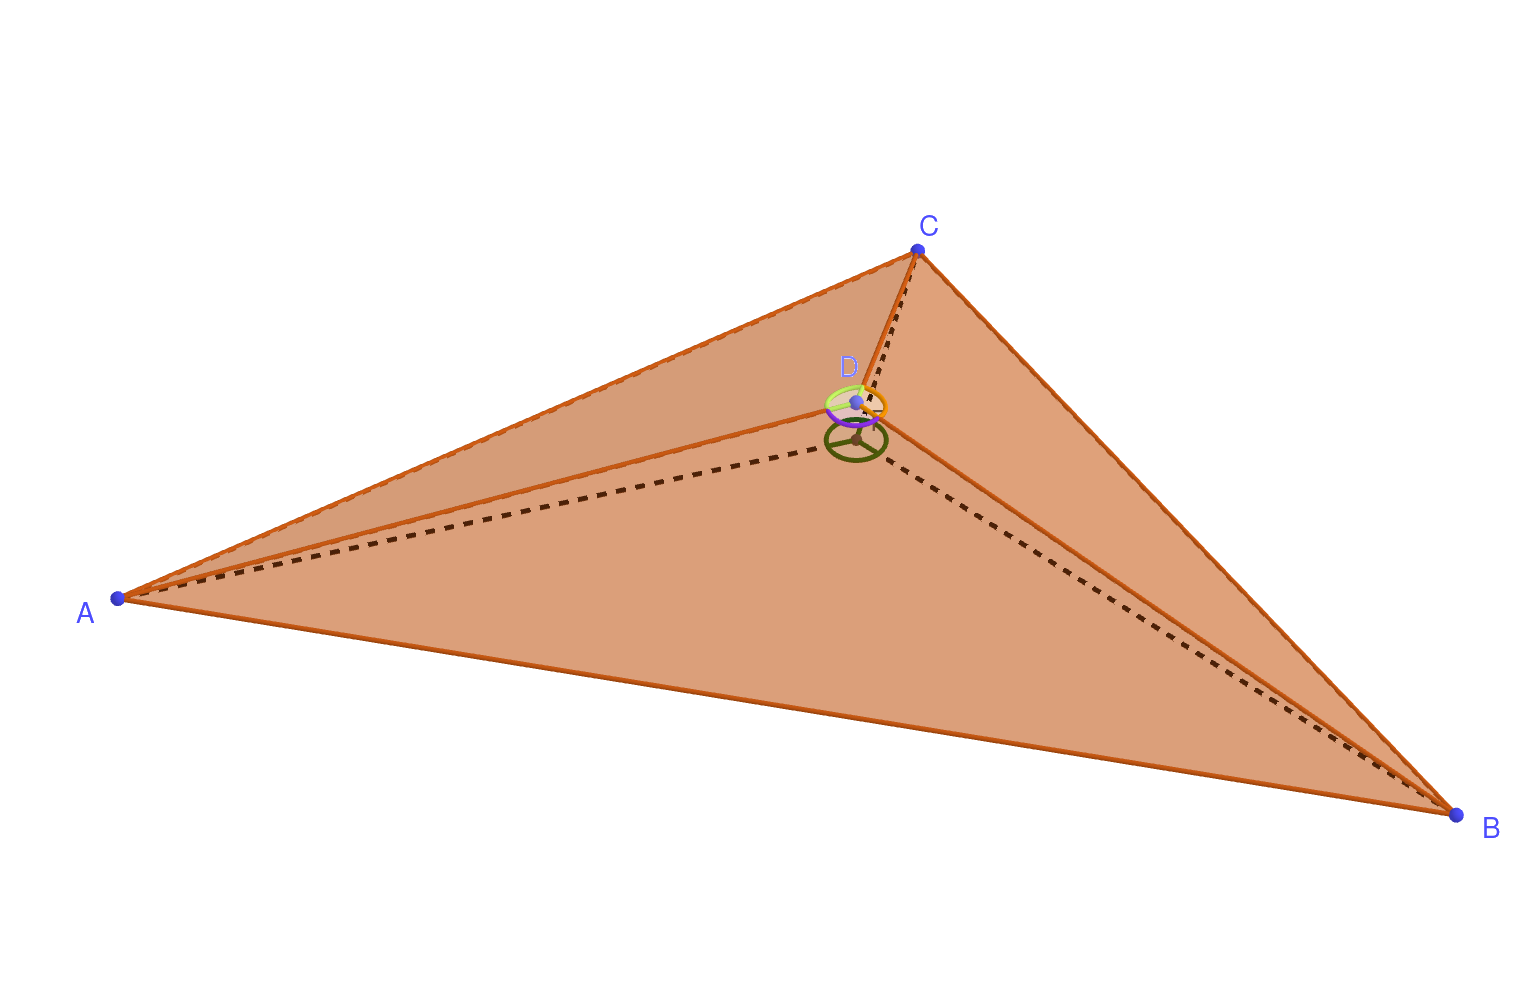
\includegraphics[scale=0.15]{img/2021_02_11/13/space.png}
\end{figure}
\subsubsection*{Zadanie~8.14.}
W~pewnym okręgu rozważmy trójkąt \(\triangle{ABC}\) wpisany w~niego. Przez punkt \(C\) poprowadźmy prostą prostopadłą do prostej \(AB\) i~oznaczmy przez \(E\) punkt jej przecięcia z~okręgiem.
\begin{figure}[H]
    \centering
    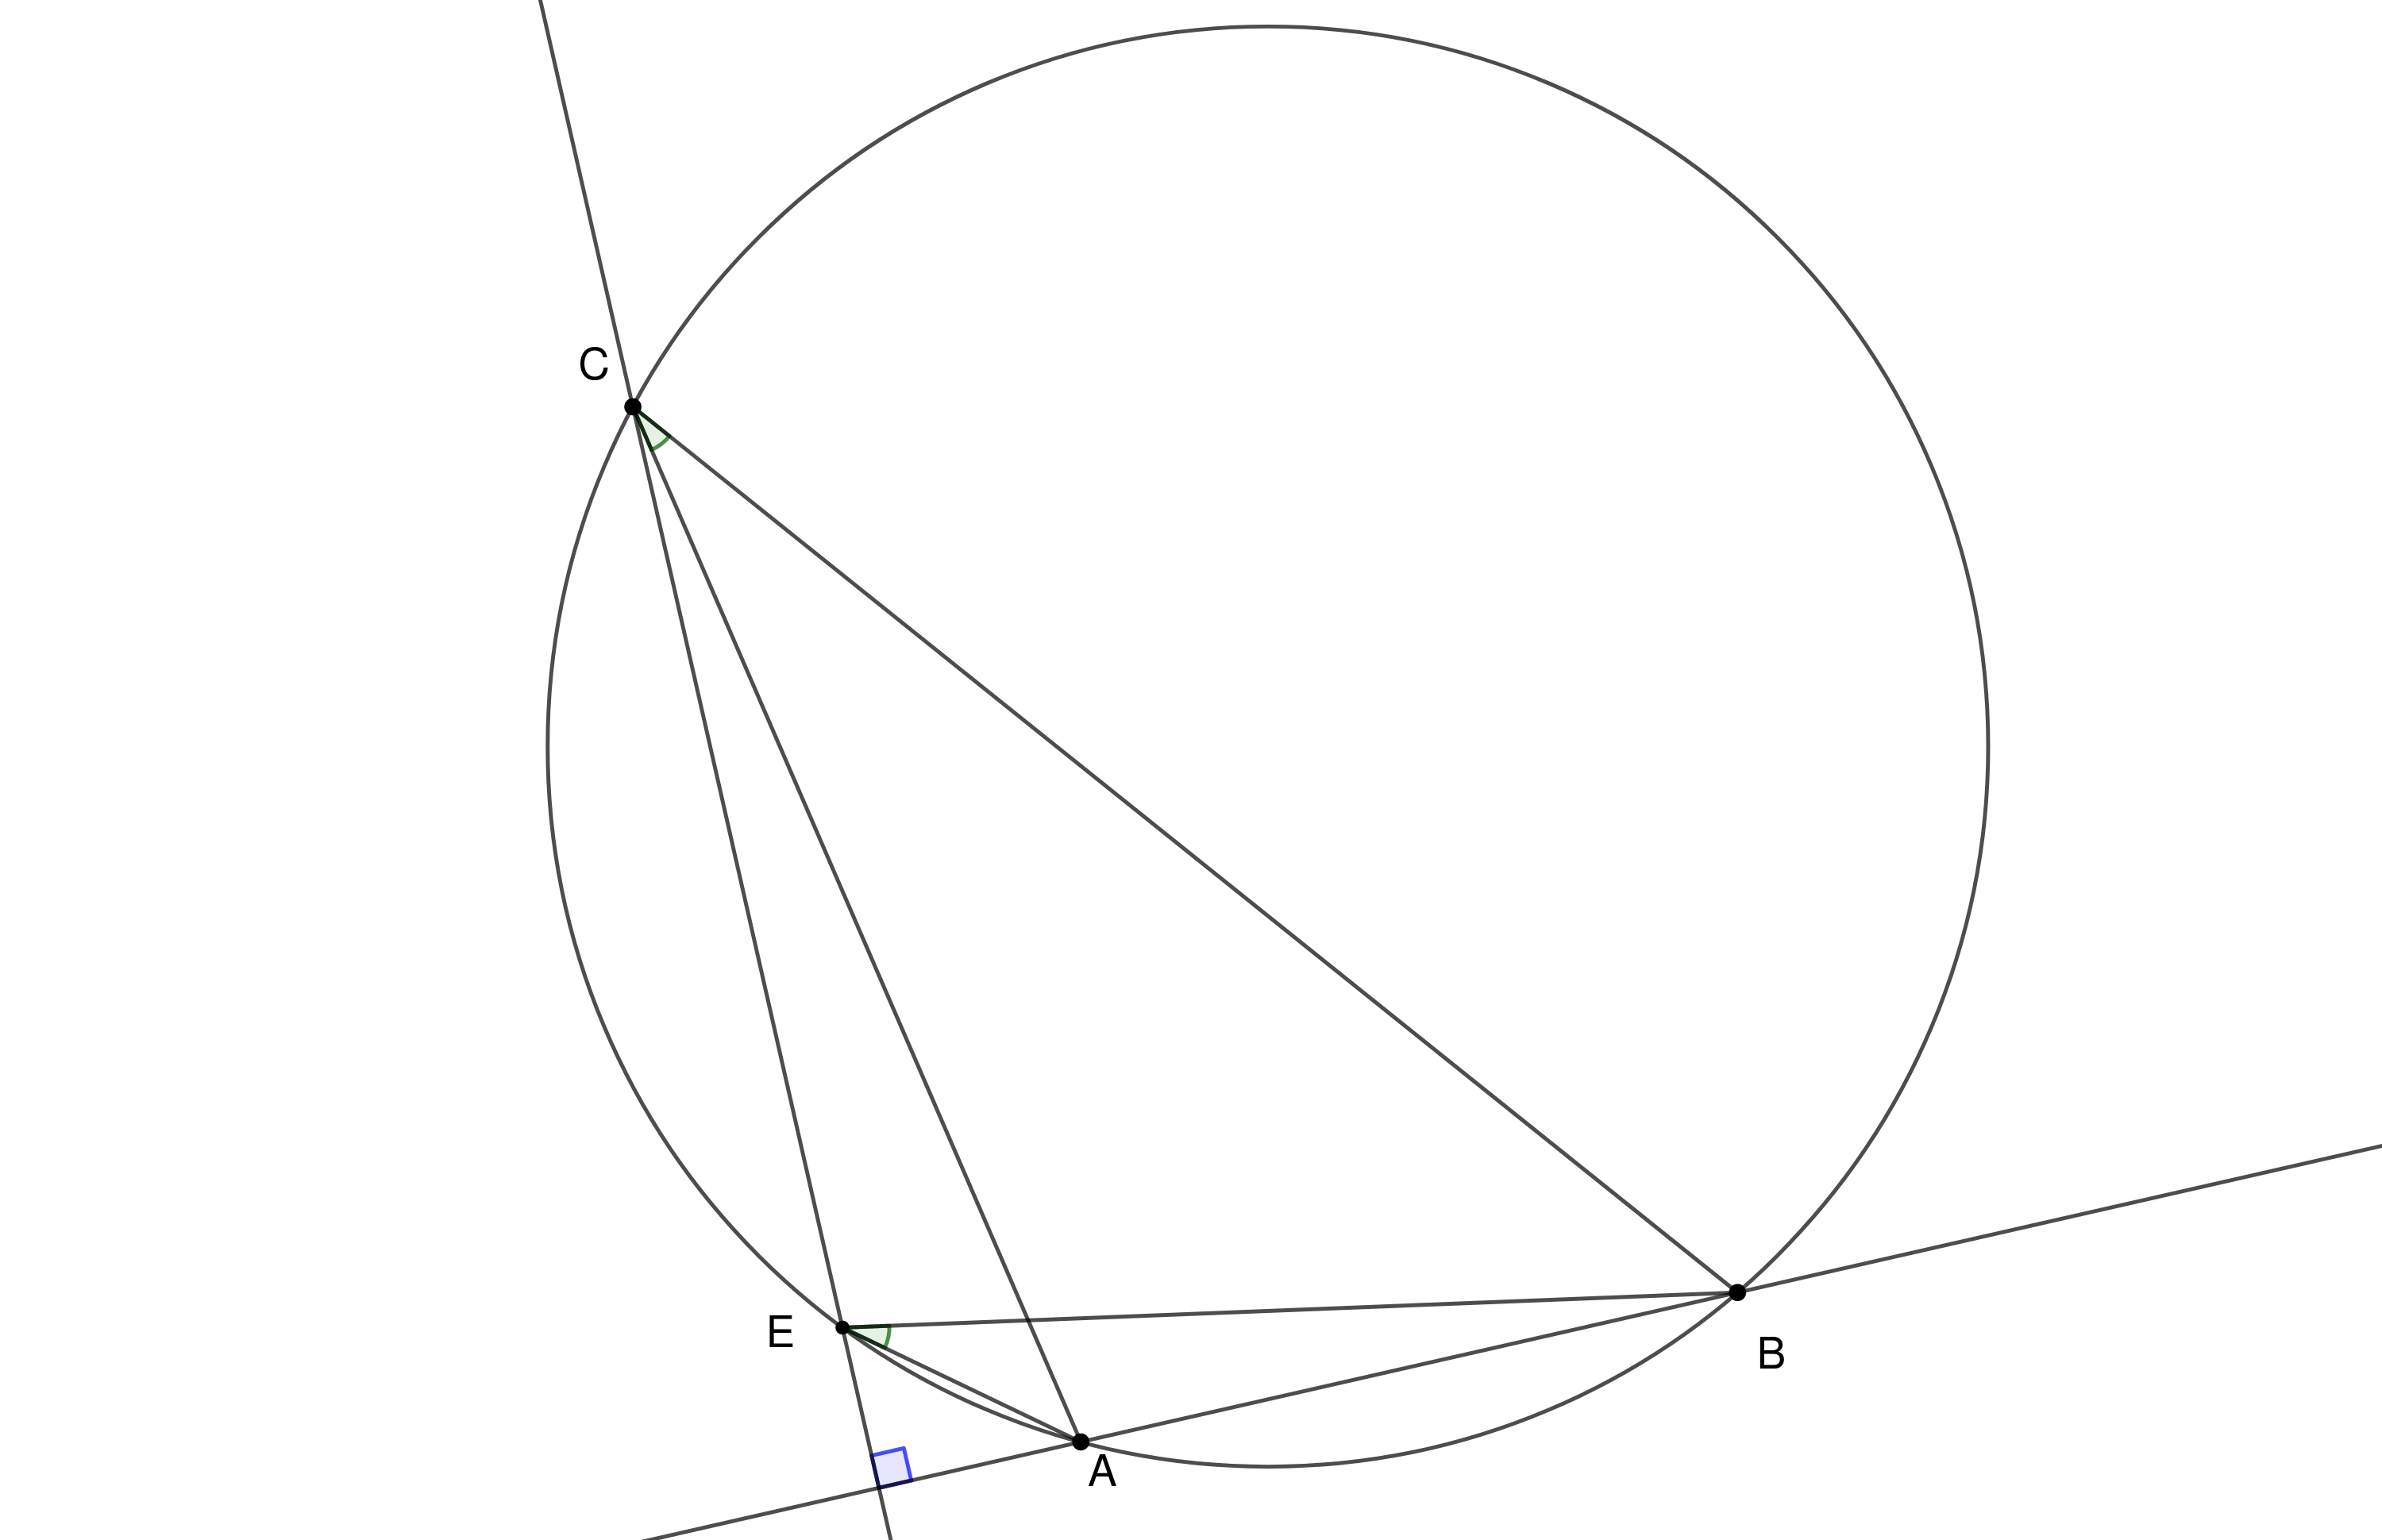
\includegraphics[width=\textwidth]{img/2021_02_11/14/plane.png}
\end{figure}
\noindent
Kąty \(\angle{ACB}\) i~\(\angle{AEB}\) mają równe miary, ponieważ są oparte na tym samym łuku. Obróćmy punkt \(E\) wokół prostej \(AB\), uzyskując w~ten sposób punkt \(D\).
\begin{figure}[H]
    \centering
    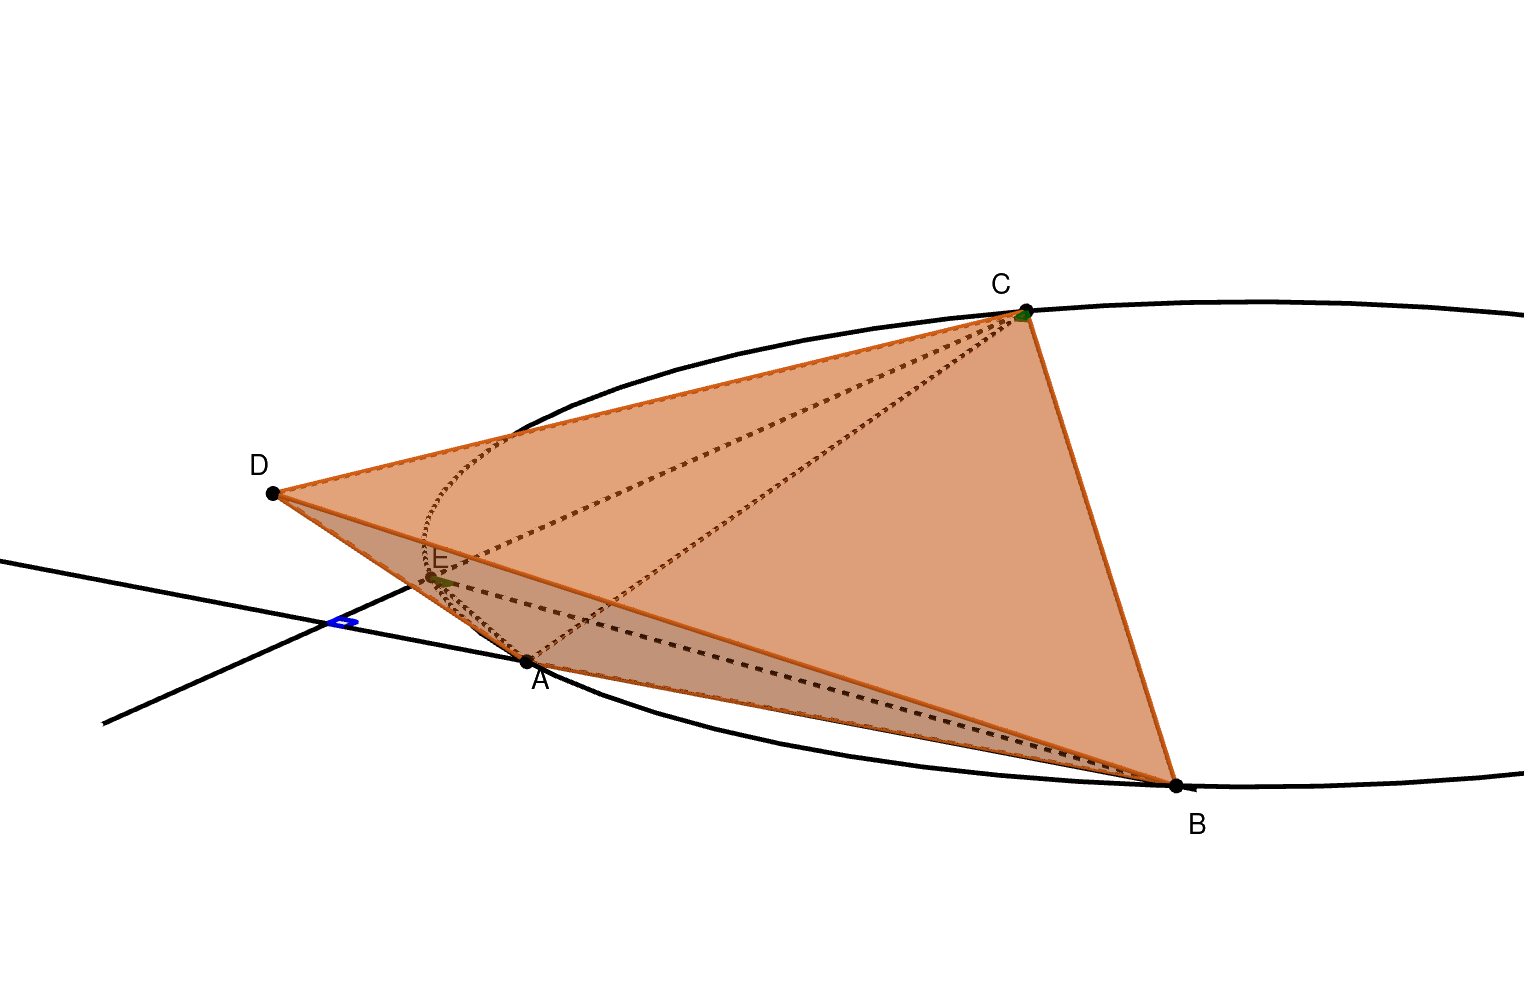
\includegraphics[scale=0.28]{img/2021_02_11/14/space.png}
\end{figure}
\noindent
Wtedy \(\triangle{ABD} \equiv \triangle{ABE}\), czyli \(\mangle{ADB} = \mangle{AEB} = \mangle{ACB}\). Wiemy też, że \(AB \perp CE\), więc \(AB \perp CD\). W~oczywisty sposób również \(\triangle{ABC} \not\equiv \triangle{ABD}\)
